\documentclass{article}

\usepackage[margin=0.7in]{geometry}
\usepackage[parfill]{parskip}
\usepackage[utf8]{inputenc}

\usepackage{graphicx} % For including images
\graphicspath{ {./images/} }
\usepackage{subcaption} % For subfigures

\usepackage{amsmath,amssymb,amsfonts,amsthm} % Math packages

\usepackage{cleveref} % Inline referencing
\usepackage[style=alphabetic]{biblatex} % For bibliography
\addbibresource{bibliography.bib}

\usepackage{setspace} % For double-spacing
\doublespacing

\newcommand\solmass{\textrm{M}_\odot}
\newcommand\kpc{\textrm{kpc}}
\newcommand\kmps{\textrm{km}/\textrm{s}}

\newcommand\vrot{\ensuremath{v_{\textrm{rot}}}}

\title{Mass Distributions of Spiral Galaxies}
\date{}

\begin{document}

\maketitle

\section{Introduction}\label{sec:introduction}

The astronomer Edwin Hubble, in a series of lectures given at Yale in 1935\footnote{These lectures were later published under the title \textit{The Realm of the Nebulae} \cite{Hubble1936}.}, provided a classification of galaxies, which he refered to as \textit{extragalactic nebulae}, into spiral and elliptic.
This classification is used even today by amateur and professional astronomers alike, though the expanded version provided by French astronomer Gérard de Vaucouleurs is preferable.
But nowadays, the morphological classification of galaxies --- classifying galaxies based on what we perceive their shape to be --- is done computationally.

\begin{figure}[h!]
    \centering
    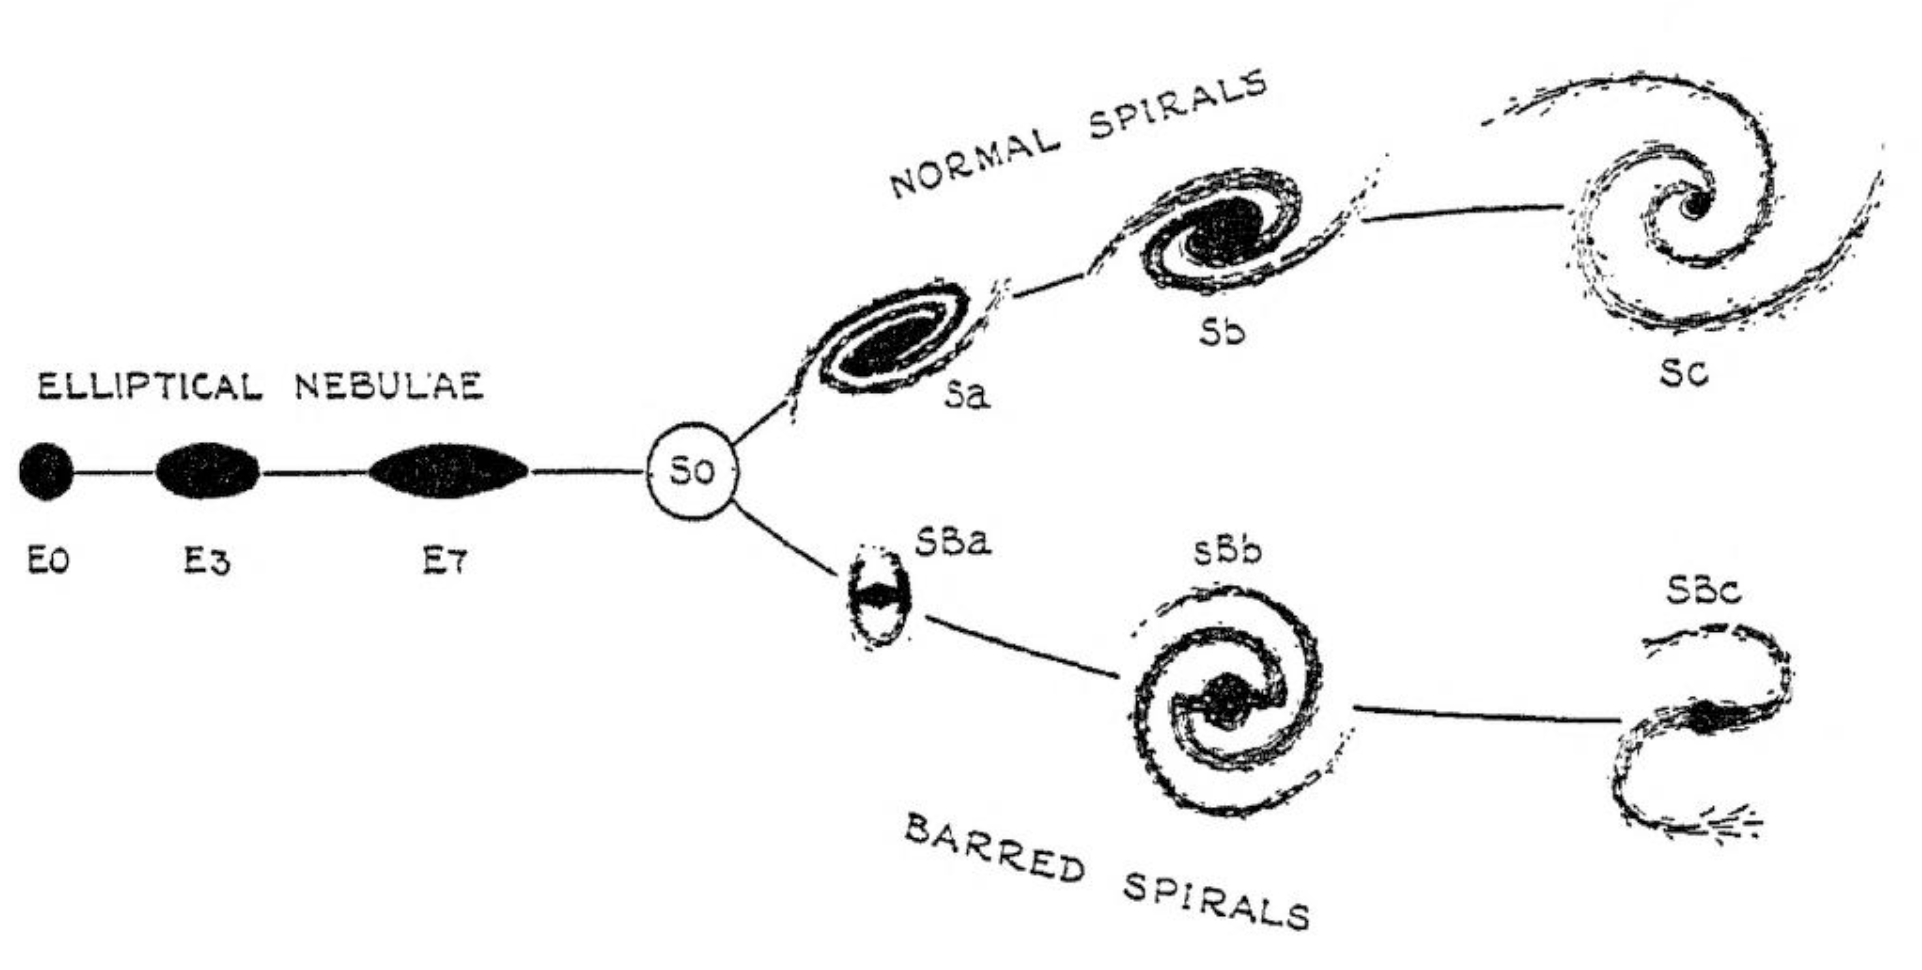
\includegraphics[width=0.7\linewidth]{hubblefork}
    \caption{Hubble's "tuning fork" classification scheme, p. 45, \cite{Hubble1936}.}
    \label{fig:hubblefork}
\end{figure}

What has enabled such computational work is the signficant progress in our ability to make precise astronomical observations over large distances and use them to make physical deductions.
One specific instance of this is the use of spectroscopy to understand the motion of galaxies relative to us, in which one measures at two seperate occassions the electromagnetic spectrum radiated by a galaxy using a \textit{spectrometer} and uses the shift observed in the emission lines to calculate the speed at which the galaxy is moving relative to us.
By making this measurement at different distances from the center of a galaxy, under the assumption that a galaxy is centrally symmetric, and accounting for the inclination possessed by the galaxy when we observe it, we can plot the \textit{rotation curve} of a galaxy; a plot of the rotational velocity against the galactocentric radius.

Since the velocity of a body in circular motion can be related to its mass using Newton's second law, I therefore explore the rotation curves of spiral galaxies under the following research question:

\begin{center}
    \textit{How is the gravitational mass of a spiral galaxy distributed within its disc, and how is this distribution determined by the rotational velocities?}
\end{center}

% \begin{itemize}
%     \item What are spiral galaxies?
%     \item Edwin Hubble's work.
%     \item What measurements have been made about spiral galaxies?
%     \item Go relatively deep; show that you've done reading outside of IB.
%     \item RQ: How is the gravitational mass of a spiral galaxy distributed within its disc, and how is this distribution determined by the rotational velocity distribution within and outside the disc?
% \end{itemize}

\section{Theory}\label{sec:theory}

Consider a spherical gas cloud of radius \(R\) and uniform density \(\rho\) that is rotating about its centre.
The rotational speed \(v_{\text{rot}}\) of a particle of mass \(m\) at distance \(r\) from the centre can be found using Newton's law of gravitation and second law of motion, which give us
\[\frac{mv_{\text{rot}}^2}{r} = \frac{GmM}{r^2},\]
or simply

\begin{equation}
    v_{\text{rot}} = \sqrt{GM/r},
    \label{eq:vrotcummass}
\end{equation}

where \(M\) is the mass of the cloud internal to the particle, naturally called the \textit{cumulative mass of the galaxy}.
Substituting

\begin{equation}\label{eq:massdense}
    M =
    \begin{cases}
        \frac{4}{3}\rho\pi r^3 & (r < R) \\
        \frac{4}{4}\rho\pi R^3 & (r \ge R)
    \end{cases}
\end{equation}

into \Cref{eq:vrotcummass} gives

\begin{equation}\label{eq:vrotdense}
    \vrot = 
    \begin{cases}
        \sqrt{\frac{G\cdot \frac 4 3 \pi \rho r^3}{r}} = \sqrt{\frac{4\rho G\pi}{3}} r & (r < R) \\
        \sqrt{\frac{G\cdot \frac 4 3 \pi \rho R^3}{r}} = \sqrt{\frac{4\rho G\pi R^3}{3}} r^{-1/2} & (r \ge R)
    \end{cases}.
\end{equation}

So for a spiral galaxy that can be accurately modelled as a spherical gas cloud of uniform density, we can graph its expected rotation curve and cumulative mass distribution as described by \Cref{eq:massdense,eq:vrotdense}; see \Cref{fig:expectedgraphs}.
Note that in this paper we use astronomical units of measurement to ease our calculations: masses are in \textit{solar masses} (\(\solmass\)), distances are in \textit{kiloparsecs} (\(\kpc\)), and velocities and speeds are in \textit{kilometers per second} (\(\kmps\)).

\begin{figure}
    \centering
    \begin{subfigure}{0.4\textwidth}
        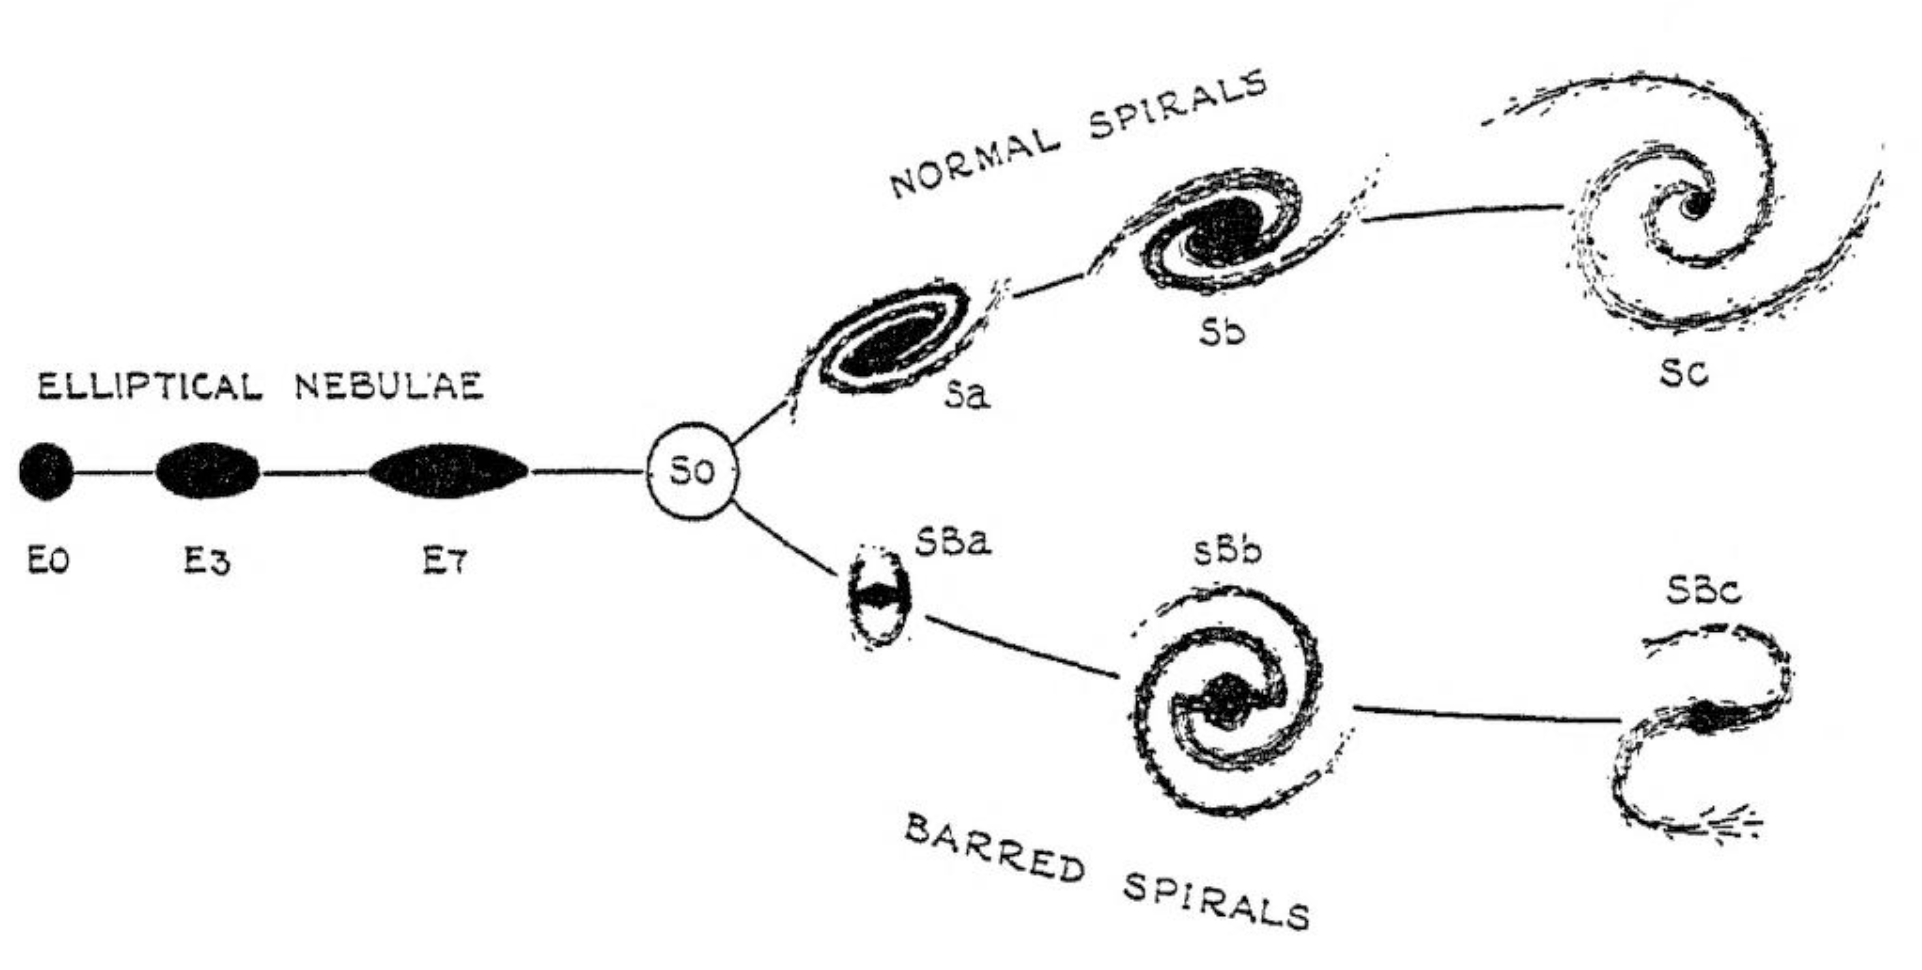
\includegraphics[width=\textwidth]{hubblefork}
        \caption{Rotation curve}
    \end{subfigure}
    \hfill
    \begin{subfigure}{0.4\textwidth}
        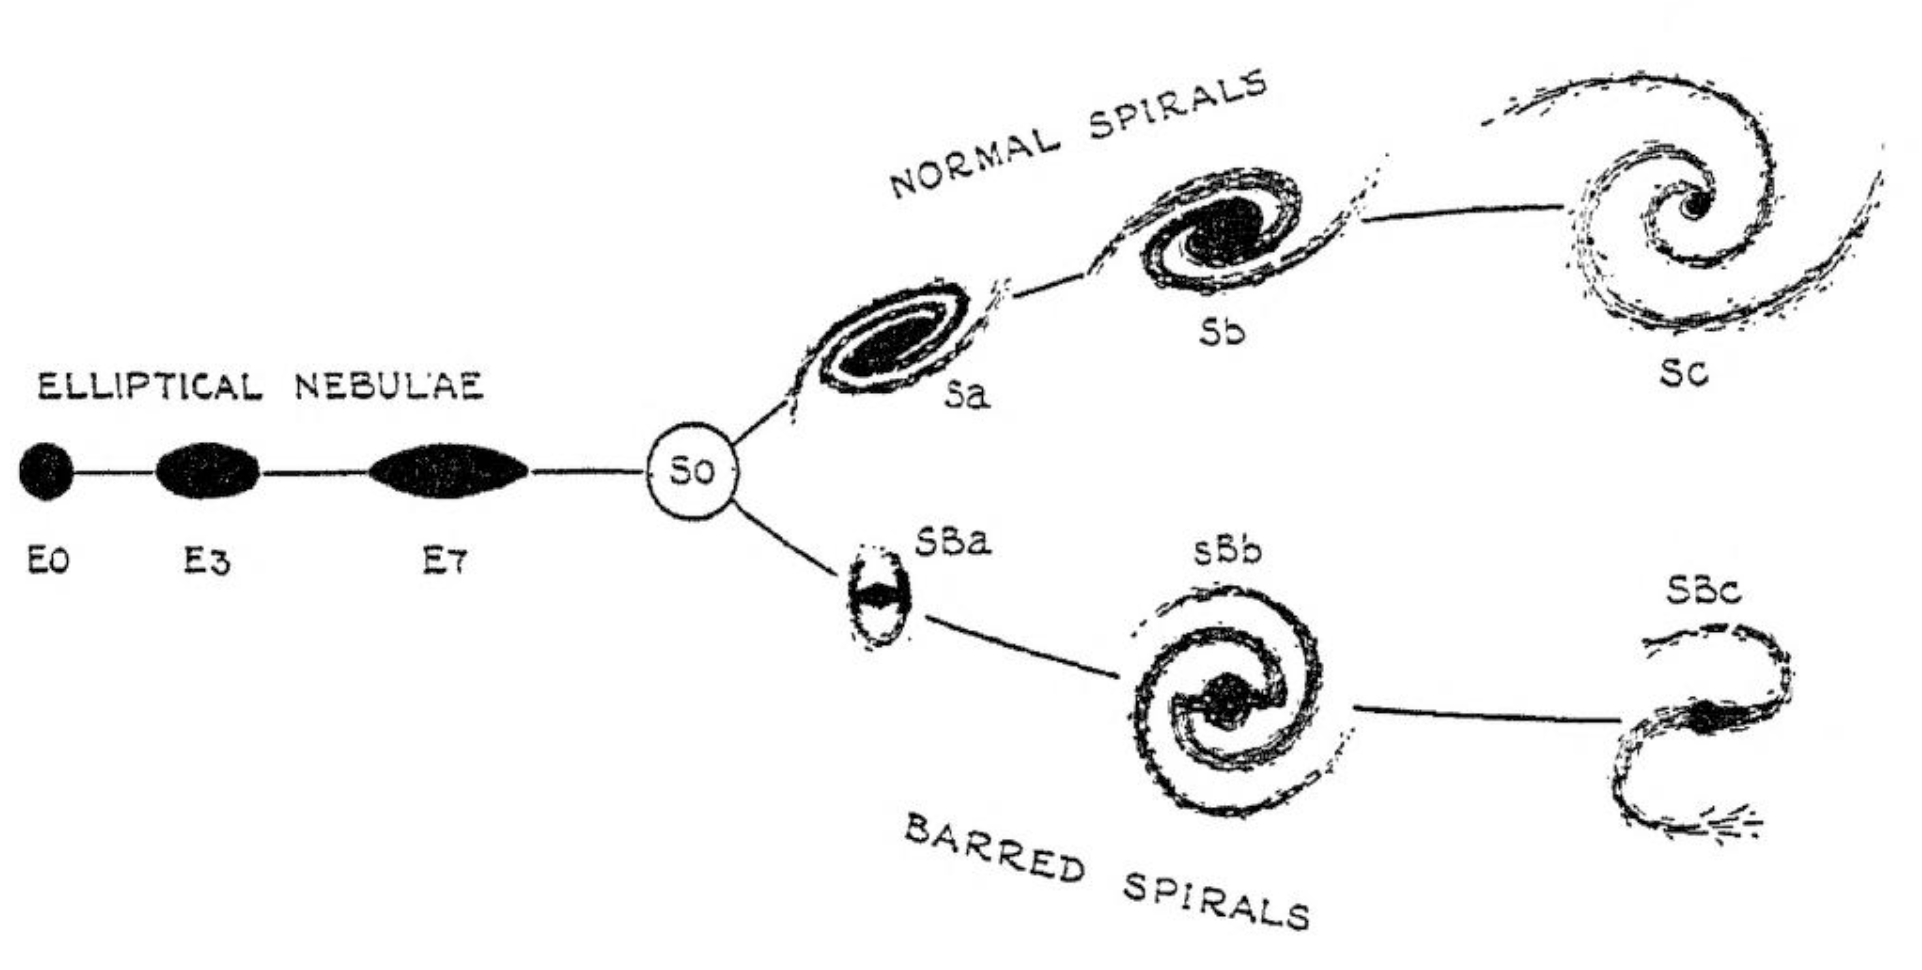
\includegraphics[width=\textwidth]{hubblefork}
        \caption{Cumulative mass distribution}
    \end{subfigure}
    \caption{Expected rotation curve and cumulative mass distribution for a galaxy.}
    \label{fig:expectedgraphs}
\end{figure}

However, as we shall see, the actual rotation curve of a spiral galaxy as well as the actual cumulative mass distribution does not look as in \Cref{fig:expectedgraphs}.

% \begin{itemize}
%     \item Number equations, to refer back to them.
%     \item Show the expected RC of a spiral galaxy.
%     \item Galaxies are usually moving away from us.
%     \item Don't say "galactocentric speed/velocity", rather "rotational speed/velocity".
% \end{itemize}

\section{Method}\label{sec:method}

This paper attempts to answer the proposed research question by analysing rotation curve data on the following galaxies: NGC0024, NGC0289, NGC1003, NGC2366, NGC2403.
The paper relies on two main sources for relevant data.
The observed velocities at various distances from the centres of these galaxies and the inclinations of the galaxies are taken from \Cite{SPARC}, which is a database of 175 spiral and irregular galaxies (including the ones mentioned above) using photometric and spectroscopic measurements from the Spitzer Space Telescope.
The chosen galaxies are all of them intentionally spiral galaxies, as the theory developed in \Cref{sec:theory} would not remain accurate for irregulars.
In addition to this database, the paper also makes use of the NASA/IPAC Extragalactic Database to ascertain the diameter of the visible disc of each of the chosen galaxies.

The paper proceeds as follows.
\Cref{sec:raw-data} tabulates all of the raw data required from the aforementioned databases; this includes the radii and inclinations of the galaxies, as well as a table for each galaxy tabulating observed velocities at different distances from the centre.
\Cref{sec:processed-data} uses this information to compute and plot the rotation curves and cumulative mass distributions of all of the galaxies.
These graphs are analysed in \Cref{sec:analysis}, and conclusions are presented in \Cref{sec:conclusion}.
Finally, \Cref{sec:evaluation} provides a brief evaluation of possible errors or inaccuracies.

\section{Raw Data}\label{sec:raw-data}

\section{Processed Data}\label{sec:processed-data}

% ---- move to METHOD

% On rearranging \Cref{eq:vrotcummass} we also find that
% 
% \begin{equation}\label{eq:internalmass}
%     M = \frac{rv_{\text{rot}}^2}{G},
% \end{equation}
% 
% allowing us to calculate the cumulative mass distribution of a galaxy, which satisfies these conditions, given its rotation curve.

% ----

\section{Analysis}\label{sec:analysis}

\section{Conclusion}\label{sec:conclusion}

\begin{itemize}
    \item Analysis provides basis for dark matter.
    \item Mention possible forms of dark matter (WIMPs, etc.)
    \item Mention alternatives to dark matter (MOND).
\end{itemize}

\section{Evaluation}\label{sec:evaluation}

\begin{itemize}
    \item Where does uncertainty come from?
    \item How does this uncertainty affect the conclusion?
\end{itemize}

% \appendix
% 
% \section{Appendix}
% 
% \subsection{Raw Data}
% 
% \begin{itemize}
%     \item Tabulate.
% \end{itemize}
% 
% \subsection{Figures}

\nocite{*}
\printbibliography

\end{document}
